\documentclass[a4paper]{article}
\usepackage[utf8]{inputenc}
\usepackage[portuguese]{babel}
\usepackage{graphicx}
\usepackage{a4wide}
\usepackage[pdftex,hidelinks]{hyperref}
\usepackage{float}
\usepackage{indentfirst}
\usepackage{subcaption}
\usepackage[cache=false]{minted}
\usepackage{amsmath}
\usepackage{listings}
\usepackage{color}

\begin{document}

\title{Processing an Angolan Newspaper}
\author{Pedro Mendes (a79003)}
\date{\today}

\begin{titlepage}

    %título
    \thispagestyle{empty}
    \begin{center}
        \begin{minipage}{0.75\linewidth}
            \centering
            %engenharia logo
            
\includegraphics[width=0.4\textwidth]{eng.jpeg}\par\vspace{1cm}
            \vspace{1.5cm}
            %títulos
            \href{https://www.uminho.pt/PT}{\scshape\LARGE Universidade do Minho} \par
            \vspace{1cm}
            \href{https://www.di.uminho.pt/}{\scshape\Large Departamento de Informática} \par
            \vspace{1.5cm}

            \maketitle
        \end{minipage}
    \end{center}

\end{titlepage}

\tableofcontents

\pagebreak

\section{Introduction}
This project aims to parse a very large file with articles from a newspaper in
order to organize them in individual articles, indexing them by title or tag.

The main tool used for the parser is \textit{flex}, (and the C programming
language) together with the \href{https://developer.gnome.org/}{GLib} library,
to produce an efficient parser. On top of this a \textit{bash} script was
written to pre-process the input file.

\section{The problem}

The input file presents a few challenges that need to be addressed.

The first and most obvious one is the file's size, it's millions of lines long
which means that the information parsed needs to be flushed as soon as it's not
needed anymore as to not risk allocating too much memory.

The second is the publication's format, which in some cases does not lend itself to clean regular expressions.

\begin{figure}[H]
    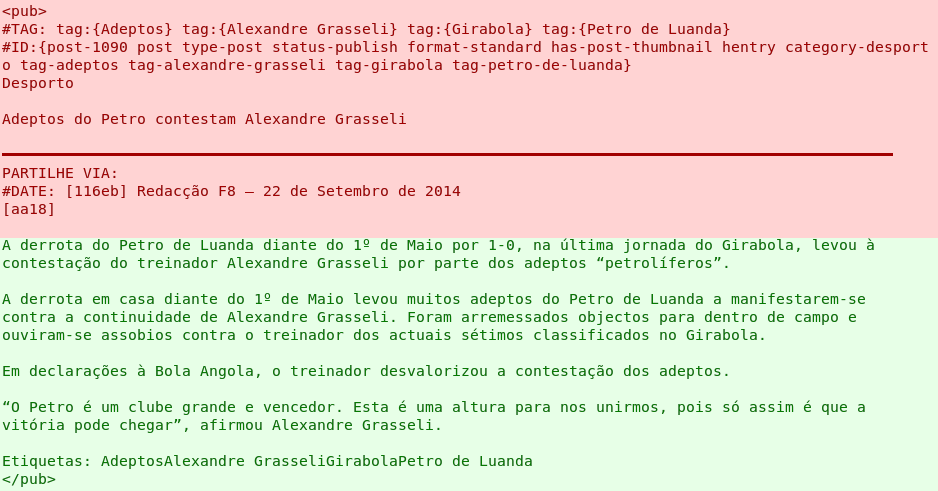
\includegraphics[width=\textwidth]{./example_pub_colored_simple.png}
    \caption{Example Publication}\label{fig:example_pub_simple}
\end{figure}

As can be seen in the example above (Figure~\ref{fig:example_pub_simple}), a
publication is split in roughly 2 parts, the header, in red, where the post's
metadata is stored and the body or text of the publication, in green. The first
area has tags, id and date which are easy to find due to their
\texttt{\#NAME\{} syntax, but the category and the title, in this example
\textit{``Desporto''} and \textit{``Adpetos de Petro contestam Alexandre
Grasseli''} respectively, have to be parsed using the rest of the header's
context. Next, sometimes there is a sequence delimited by square brackets before
the text, this is also intended to be eliminated.

The third and final problem to be addressed is the fact that most publications
are repeated throughout the file which can interfere with the counting of the
number of occurrences of each tag.

\section{Solution}

\section{Project Architecture}

Handling of the parsed information is split in two modules, \texttt{publication} and \texttt{newspaper}.

\subsection{Publication}

This module gathers the information of a single publication to create the
corresponding \texttt{post-id.html} file. When a publication is found this
module is initialized and, as the parser runs, this structure accumulates the
\texttt{id}, \texttt{title}, \texttt{author\_date}, \texttt{category} and
\texttt{tags}, then after the header is flushed to the post file, the body of
the publication is immediately flushed to the file as to not accumulate to many
bytes in memory.

\subsection{Newspaper}

%%TODO: Rewrite this paragraph
This module indexes the posts and their tags to create the final \texttt{index.html}, \texttt{tags.html} and individual tag files. The first one contains a link to every post and a link to the tags file, which in turn has a list of all the tags and how many times it occurs. A link to a tag is the equivalent of saying a link to a list of posts with said tag. In order to build this file two tables are kept in memory, one associates post id with it's title and tags, the other one associates tags with the posts where they were found. This way it's possible to cross reference posts and tags. After the parsing is done the index and tags files are created. The tags files

\section{Conclusion}

\end{document}

